\chapter{Introduction}
\label{chap:chapter1}
\pagenumbering{arabic}\hspace{3mm}

The basic job of a compiler is code translation from a high level 
language to a target assembly language. But, compilers also run
multiple optimization pass in the intermediate stages of translation, 
so that the finally generated code performs better than just a normal 
translated code. There might be a one time overhead of 
running optimizations, but the performance gain visible over multiple 
executions of the code outweighs it.

Modern compilers performs a large number of optimizations like
induction variable analysis, loop interchange, loop invariant code
motion, loop unrolling, global value numbering, dead code 
optimizations, constant folding and propagation, common subexpression 
elimination etc. One common feature of most of these optimizations is 
detecting equivalent program subexpressions. 

Checking equivalence of program subexpressions has been shown to be 
an undecidable problem, even when all the conditional statements are 
considered as non deterministic. So, in most of the cases compilers 
try to find some restricted form of expression equivalence. One such
form of expression equivalence is called  \textit{Herbrand 
Equivalence} (see below).
Detecting equivalence of program subexpressions can be used for 
variety of applications. Compilers can use these to perform several 
of the optimizations mentioned above like constant propagation, 
common subexpression elimination etc. Program verification tools can 
use these equivalences to discover loop invariants and to verify 
program assertions. This information is also important for discovering
equivalent computations in different programs, which can be used by
plagiarism detection tools and translation validation tools \cite
{Necula, Pnueli}, which compare a program with an optimized version
in order to check correctness of the optimizer.


\section{Herbrand Equivalence}
A formal definition of Herbrand Equivalence is given in \cite{Ruthing}.
Informally, two expressions are Herbrand equivalent at a program 
point, if and only if they have syntactically the same value at that 
particular point, across all the execution paths from the start of 
the program which reaches that point. For the purpose of analysis, 
the operators themselves are treated as uninterprated functions with 
no semantic significance, only syntactic information is taken into 
consideration.

For Herbrand equivalence analysis, we consider the set of all 
possible expressions that can be formed using the constants, 
variables and operators used in the program. And for each program 
point, partition them such that two expressions are Herbrand 
equivalent at that point if and only if they belong to the same 
partition class for that point.

\begin{figure}[!ht]
    \centering {
        \setlength{\fboxsep}{8pt}    
        \fbox{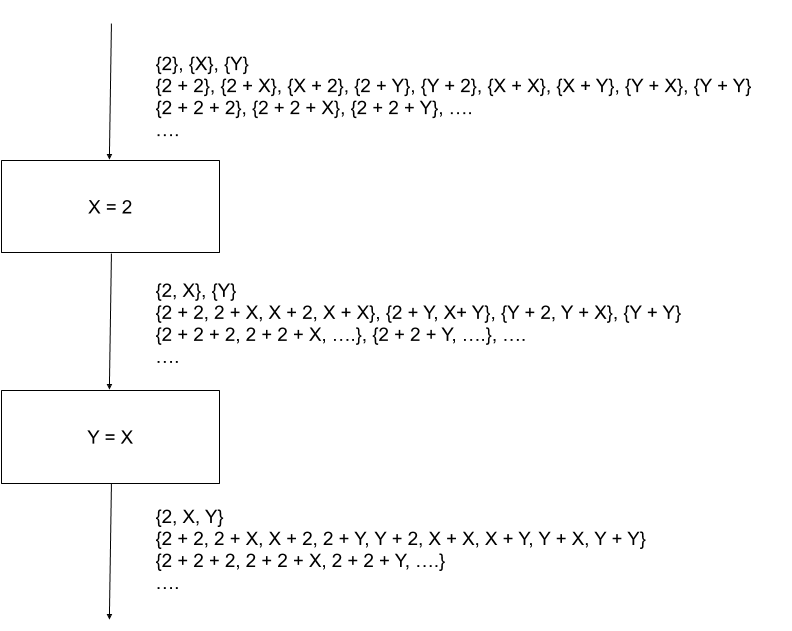
\includegraphics[scale=0.5]{HerbrandEquivalenceTrans.png}}
    }
    \caption{Example of Herbrand Equivalence}
    \label{fig:herbrandExampleTrans}
\end{figure}

Figure \ref{fig:herbrandExampleTrans} shows a simple example of Herbrand Equivalence analysis. All the expressions that belongs to the same set at a program point are Herbrand equivalent at that point.
\begin{itemize}
    \item   Initially all the expressions are in separate sets, ie. 
    they are inequivalent to each other. In particular, note that 
    $X + 2$ and $2 + X$ are inequivalent because the operators are 
    being treated uninterprated with no semantic information of them, 
    which means there is no knowledge of commutativity of $+$.
    \item   After assignment $X = 1$, any occurrence of $X$ in an
    expression can be replaced with $1$. So, now all expressions with 
    $1$ in place of $X$ and vice versa are equivalent.
    \item   After assignment $Y = X$, any occurrence of $Y$ in 
    an expression can be replaced with $X$. Because $X$ and $1$ are 
    equivalent, it means now $1$, $X$, and $Y$ are all equivalent to 
    each other. And two expressions are equivalent if one can be 
    obtained from the other by replacing one of these with any of the 
    other two. For this example, it means that two expressions of 
    the same length are equivalent.
\end{itemize}

\begin{figure}[!ht]
    \centering {
        \setlength{\fboxsep}{8pt}    
        \fbox{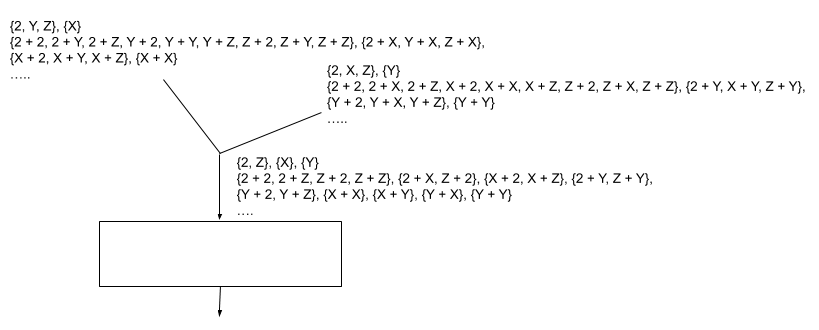
\includegraphics[scale=0.5]{HerbrandEquivalenceConv.png}}
    }
    \caption{Example of Herbrand Equivalence analysis at a confluence point}
    \label{fig:herbrandExampleConv}
\end{figure}

Figure \ref{fig:herbrandExampleConv} shows what happens at a \textit
{confluence point} - a point where multiple paths meet. Two 
expressions are Herbrand equivalent only if they are Herbrand 
equivalent at all the predecessor points.
\begin{itemize}
    \item   In the left branch $2$, $Y$, $Z$ are equivalent and 
    so are expressions obtained by replacement of any of these with any other.
    \item   The case with the right branch is similar, except $X$ and $Y$ are interchanged.
    \item   At the confluence point, only $2$ and $Z$ are equivalent 
    because they were equivalent at both the predecessors points. $X$ 
    was equivalent to $2$ and $Z$ at the right predecessor but not 
    the left one and $Y$ was equivalent to $2$ and $Z$ at the left 
    predecessor but not the right. As before, expressions obtained by 
    replacing $2$ with $Z$ and vice versa are equivalent.
\end{itemize}


\section{Organization of The Report}
Chapter \ref{chap:chapter2} gives a brief overview of previous works 
related to the Herbrand Equivalence. Then a brief summary of the 
papers \cite{Gulwani, Saleena, Babu} is presented. Chapter 
\ref{chap:chapter6} provides a tutorial on writing an LLVM 
optimzation pass. Finally, chapter \ref{chap:chapter7} gives a 
pseudocode for Herbrand Equivalence analysis of a program, which 
is based on the algorithm mentioned in \cite{Babu}.

